\section{Introduction}

Evolutionary computation researchers have devoted a great deal of attention to understanding how to promote stable coexistence between lineages exploring different regions of a fitness landscape. By definition, any processes that promote this behavior would be classified by biologists as ecological dynamics: effects of short time-scale interactions between individuals that are not closely related. Ecologists have developed robust mathematical models to explain the precise parameter ranges under which different species can stably coexist. While translating these results to evolving systems is challenging due to the resulting eco-evolutionary feedback loops,  it has the potential to clarify important unresolved questions about ecological dynamics used in evolutionary computation. 

Promoting diversity within an evolving population is important for evolutionary computation because it encourages exploration of a higher percentage of the fitness landscape and reduces the chances of premature convergence on a suboptimal fitness peak. However, some types of diversity facilitate finding the global optimum better than other types. For instance, increasing the mutation rate generates more new genotypes but is unlikely to meaningfully increase the spread of the population across the fitness landscape. Even amongst more advanced approaches to generating and maintaining diversity, some seem to systematically produce diversity that is spread across the fitness landscape in ways that are more conducive to solving a given problem than the diversity produced by other approaches. We hypothesize that a better mechanistic understanding of the underlying ecological dynamics will facilitate making better choices about which approach is most appropriate for which problems (this applies both to low-level choices like parameter settings and high-level choices like which selection mechanism to use). Additionally, by clarifying which aspects of existing algorithms are driving the desired results, we may be able to design more effective variations on them.


\subsection{Primer on coexistence theory}

- Niches based on climatic tolerance vs. niches based on outcompeting others when resource is present.

- Resources = public goods. Using them harms all others that could use them

- hypothesized ideal characteristics for EC

- how various selection schemes fit into ecology
- Fitness sharing

\subsection{Lexicase Selection}
In lexicase selection, a large number of criteria are chosen for solutions to be evaluated on. Traditionally, these criteria are each individual test cases, but recent work suggests that other types of fitness functions are also effective [CITE GPTP paper?]. Every time an individual is selected to reproduce, the selection criteria are randomly reordered. The entire population is evaluated on the first one. The individuals that perform best on this first criterion are then evaluated on the second criterion. The ones that perform best on that criterion are then evaluated on the third, and so on, until only one individual remains or all criteria have been used and the winner is selection randomly from the remaining options.

In ecological terms, this creates a vast number of niches nested within each other. While it is tempting to use a resource metaphor to understand the competition within these niches, this is actually incorrect and misleading. Whereas using a resource harms all others that use that resource, improving on a selection criterion in lexicase selection only harms a (usually small) subset of the population. Instead, we argue that population structure is a better metaphor for lexicase selection. Imagine $N!$ islands, where each island corresponds to a single potential ordering of selection criteria and can only be inhabited by the individuals that are best at that ordering. Each island has a fixed amount of space. This is analagous to situations in nature where niches are defined exclusively by ability to survive a set of abiotic conditions. Being better able to survive these conditions increases the number of offspring an individual can have. Over time, genotypes that are better at surviving in a given set of conditions competitively exclude those that are worse. In the case of lexicase selection, this competitive exclusion happens more rapidly than it usually would in biology, but the principle is the same. 

- Mention weird thing about all space being adjacent

$N!$ is the maximum number of genotypes that should be able to stably coexist in the long term within a population under lexicase selection. While islands can potentially be inhabited by multiple genotypes that are equally able to occupy it, this coexistence will be unstable if neither genotype has another island to itself. The instability results from the fact that, within a single island, each genotype has equal fitness and competes with itself the same amount that it competes with other genotypes on the island. Thus, as stated in equation [EQUATION], there is no stabilizing pressure to increase the populations of rare genotypes within an island. Eventually, all but one should stochastically go extinct.

Because of the laws of probability, this coexistence is not technically permanent. Orderings are selected randomly, and there is always a chance that a given one will not be selected on a given generation. However, as the number of solutions that can live on each island ($\frac{population}{N!}$) increases, the odds of a catastrophic event that wipes out a whole island decrease rapidly. We can extend this rule to also cover the many cases where the total population size is less than the number of islands (i.e. islands can support less than one individual each). In these cases, it is no longer sufficient to control a single island. Instead, we calculate the sum of the total controlled area (counting fractions of islands, in the case of ties). This process produces a single number, $w$ for each genotype, indicating what fraction of the total space it controls. We use the variable $w$ here for consistency with biological theory, because this value also corresponds to an individual's probability of being selected, i.e. its biological fitness. Just as species in nature face greater risk of stochastic extinction of their range (the area they inhabit) is too small, so too do genotypes in lexicase selection. The chances of surviving for $G$ generations are given by the equation:

\begin{equation}
(1 - (1-w)^{population size})^{G}
\end{equation}
Plotting these functions, we can see that 

The selection criteria determine which other individuals in the population a given solution is competeing with for space. 

\subsection{MAP-Elites}


\subsection{Eco-EA}
Developed by Goings and Ofria, Eco-EA is an approach to solving complex problems by associating limited resources with solving various components of the larger problem. When a population first solves a sub-task, the associated resource is plentiful and the individuals capable of using it are very successful. As the number of individuals using the resource increases, it become less valuable. 

\section{Methods}

\section{Results and Discussion}

\section{Conclusion}


\subsection{Citations}
Citations to articles~\cite{bowman:reasoning,
clark:pct, braams:babel, herlihy:methodology},
conference proceedings~\cite{clark:pct} or maybe
books \cite{Lamport:LaTeX, salas:calculus} listed
in the Bibliography section of your
article will occur throughout the text of your article.
You should use BibTeX to automatically produce this bibliography;
you simply need to insert one of several citation commands with
a key of the item cited in the proper location in
the \texttt{.tex} file~\cite{Lamport:LaTeX}.
The key is a short reference you invent to uniquely
identify each work; in this sample document, the key is
the first author's surname and a
word from the title.  This identifying key is included
with each item in the \texttt{.bib} file for your article.

The details of the construction of the \texttt{.bib} file
are beyond the scope of this sample document, but more
information can be found in the \textit{Author's Guide},
and exhaustive details in the \textit{\LaTeX\ User's
Guide} by Lamport~\shortcite{Lamport:LaTeX}.

This article shows only the plainest form
of the citation command, using \texttt{{\char'134}cite}.

Some examples.  A paginated journal article \cite{Abril07}, an enumerated
journal article \cite{Cohen07}, a reference to an entire issue \cite{JCohen96},
a monograph (whole book) \cite{Kosiur01}, a monograph/whole book in a series (see 2a in spec. document)
\cite{Harel79}, a divisible-book such as an anthology or compilation \cite{Editor00}
followed by the same example, however we only output the series if the volume number is given
\cite{Editor00a} (so Editor00a's series should NOT be present since it has no vol. no.),
a chapter in a divisible book \cite{Spector90}, a chapter in a divisible book
in a series \cite{Douglass98}, a multi-volume work as book \cite{Knuth97},
an article in a proceedings (of a conference, symposium, workshop for example)
(paginated proceedings article) \cite{Andler79}, a proceedings article
with all possible elements \cite{Smith10}, an example of an enumerated
proceedings article \cite{VanGundy07},
an informally published work \cite{Harel78}, a doctoral dissertation \cite{Clarkson85},
a master's thesis: \cite{anisi03}, an online document / world wide web
resource \cite{Thornburg01, Ablamowicz07, Poker06}, a video game (Case 1) \cite{Obama08} and (Case 2) \cite{Novak03}
and \cite{Lee05} and (Case 3) a patent \cite{JoeScientist001},
work accepted for publication \cite{rous08}, 'YYYYb'-test for prolific author
\cite{SaeediMEJ10} and \cite{SaeediJETC10}. Other cites might contain
'duplicate' DOI and URLs (some SIAM articles) \cite{Kirschmer:2010:AEI:1958016.1958018}.
Boris / Barbara Beeton: multi-volume works as books
\cite{MR781536} and \cite{MR781537}.

A couple of citations with DOIs: \cite{2004:ITE:1009386.1010128,
  Kirschmer:2010:AEI:1958016.1958018}. 

Online citations: \cite{TUGInstmem, Thornburg01, CTANacmart}.  


\subsection{Tables}
Because tables cannot be split across pages, the best
placement for them is typically the top of the page
nearest their initial cite.  To
ensure this proper ``floating'' placement of tables, use the
environment \textbf{table} to enclose the table's contents and
the table caption.  The contents of the table itself must go
in the \textbf{tabular} environment, to
be aligned properly in rows and columns, with the desired
horizontal and vertical rules.  Again, detailed instructions
on \textbf{tabular} material
are found in the \textit{\LaTeX\ User's Guide}.

Immediately following this sentence is the point at which
Table~\ref{tab:freq} is included in the input file; compare the
placement of the table here with the table in the printed
output of this document.

\begin{table}
  \caption{Frequency of Special Characters}
  \label{tab:freq}
  \begin{tabular}{ccl}
    \toprule
    Non-English or Math&Frequency&Comments\\
    \midrule
    \O & 1 in 1,000& For Swedish names\\
    $\pi$ & 1 in 5& Common in math\\
    \$ & 4 in 5 & Used in business\\
    $\Psi^2_1$ & 1 in 40,000& Unexplained usage\\
  \bottomrule
\end{tabular}
\end{table}

To set a wider table, which takes up the whole width of the page's
live area, use the environment \textbf{table*} to enclose the table's
contents and the table caption.  As with a single-column table, this
wide table will ``float'' to a location deemed more desirable.
Immediately following this sentence is the point at which
Table~\ref{tab:commands} is included in the input file; again, it is
instructive to compare the placement of the table here with the table
in the printed output of this document.


\begin{table*}
  \caption{Some Typical Commands}
  \label{tab:commands}
  \begin{tabular}{ccl}
    \toprule
    Command &A Number & Comments\\
    \midrule
    \texttt{{\char'134}author} & 100& Author \\
    \texttt{{\char'134}table}& 300 & For tables\\
    \texttt{{\char'134}table*}& 400& For wider tables\\
    \bottomrule
  \end{tabular}
\end{table*}
% end the environment with {table*}, NOTE not {table}!

It is strongly recommended to use the package booktabs~\cite{Fear05}
and follow its main principles of typography with respect to tables:
\begin{enumerate}
\item Never, ever use vertical rules.
\item Never use double rules.
\end{enumerate}
It is also a good idea not to overuse horizontal rules.


\subsection{Figures}

Like tables, figures cannot be split across pages; the best placement
for them is typically the top or the bottom of the page nearest their
initial cite.  To ensure this proper ``floating'' placement of
figures, use the environment \textbf{figure} to enclose the figure and
its caption.

This sample document contains examples of \texttt{.eps} files to be
displayable with \LaTeX.  If you work with pdf\LaTeX, use files in the
\texttt{.pdf} format.  Note that most modern \TeX\ systems will convert
\texttt{.eps} to \texttt{.pdf} for you on the fly.  More details on
each of these are found in the \textit{Author's Guide}.

\begin{figure}

\includegraphics{fly}
\caption{A sample black and white graphic.}
\end{figure}

\begin{figure}

\includegraphics[height=1in, width=1in]{fly}
\caption{A sample black and white graphic
that has been resized with the \texttt{includegraphics} command.}
\end{figure}


As was the case with tables, you may want a figure that spans two
columns.  To do this, and still to ensure proper ``floating''
placement of tables, use the environment \textbf{figure*} to enclose
the figure and its caption.  And don't forget to end the environment
with \textbf{figure*}, not \textbf{figure}!

\begin{figure*}
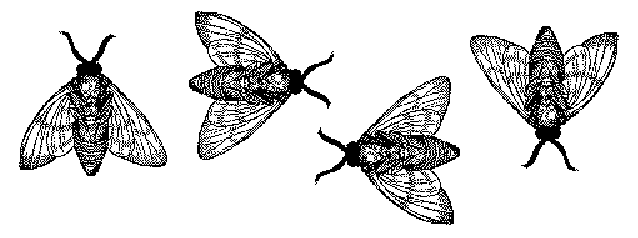
\includegraphics{flies}
\caption{A sample black and white graphic
that needs to span two columns of text.}
\end{figure*}


\begin{figure}

\includegraphics[height=1in, width=1in]{rosette}
\caption{A sample black and white graphic that has
been resized with the \texttt{includegraphics} command.}
\end{figure}

\subsection{Theorem-like Constructs}

Other common constructs that may occur in your article are the forms
for logical constructs like theorems, axioms, corollaries and proofs.
ACM uses two types of these constructs:  theorem-like and
definition-like.

Here is a theorem:
\begin{theorem}
  Let $f$ be continuous on $[a,b]$.  If $G$ is
  an antiderivative for $f$ on $[a,b]$, then
  \begin{displaymath}
    \int^b_af(t)\,dt = G(b) - G(a).
  \end{displaymath}
\end{theorem}

Here is a definition:
\begin{definition}
  If $z$ is irrational, then by $e^z$ we mean the
  unique number that has
  logarithm $z$:
  \begin{displaymath}
    \log e^z = z.
  \end{displaymath}
\end{definition}

The pre-defined theorem-like constructs are \textbf{theorem},
\textbf{conjecture}, \textbf{proposition}, \textbf{lemma} and
\textbf{corollary}.  The pre-defined de\-fi\-ni\-ti\-on-like constructs are
\textbf{example} and \textbf{definition}.  You can add your own
constructs using the \textsl{amsthm} interface~\cite{Amsthm15}.  The
styles used in the \verb|\theoremstyle| command are \textbf{acmplain}
and \textbf{acmdefinition}.

Another construct is \textbf{proof}, for example,

\begin{proof}
  Suppose on the contrary there exists a real number $L$ such that
  \begin{displaymath}
    \lim_{x\rightarrow\infty} \frac{f(x)}{g(x)} = L.
  \end{displaymath}
  Then
  \begin{displaymath}
    l=\lim_{x\rightarrow c} f(x)
    = \lim_{x\rightarrow c}
    \left[ g{x} \cdot \frac{f(x)}{g(x)} \right ]
    = \lim_{x\rightarrow c} g(x) \cdot \lim_{x\rightarrow c}
    \frac{f(x)}{g(x)} = 0\cdot L = 0,
  \end{displaymath}
  which contradicts our assumption that $l\neq 0$.
\end{proof}

\section{Conclusions}
This paragraph will end the body of this sample document.
Remember that you might still have Acknowledgments or
Appendices; brief samples of these
follow.  There is still the Bibliography to deal with; and
we will make a disclaimer about that here: with the exception
of the reference to the \LaTeX\ book, the citations in
this paper are to articles which have nothing to
do with the present subject and are used as
examples only.
%\end{document}  % This is where a 'short' article might terminate



\appendix
%Appendix A
\section{Headings in Appendices}
The rules about hierarchical headings discussed above for
the body of the article are different in the appendices.
In the \textbf{appendix} environment, the command
\textbf{section} is used to
indicate the start of each Appendix, with alphabetic order
designation (i.e., the first is A, the second B, etc.) and
a title (if you include one).  So, if you need
hierarchical structure
\textit{within} an Appendix, start with \textbf{subsection} as the
highest level. Here is an outline of the body of this
document in Appendix-appropriate form:
\subsection{Introduction}
\subsection{The Body of the Paper}
\subsubsection{Type Changes and  Special Characters}
\subsubsection{Math Equations}
\paragraph{Inline (In-text) Equations}
\paragraph{Display Equations}
\subsubsection{Citations}
\subsubsection{Tables}
\subsubsection{Figures}
\subsubsection{Theorem-like Constructs}
\subsubsection*{A Caveat for the \TeX\ Expert}
\subsection{Conclusions}
\subsection{References}
Generated by bibtex from your \texttt{.bib} file.  Run latex,
then bibtex, then latex twice (to resolve references)
to create the \texttt{.bbl} file.  Insert that \texttt{.bbl}
file into the \texttt{.tex} source file and comment out
the command \texttt{{\char'134}thebibliography}.
% This next section command marks the start of
% Appendix B, and does not continue the present hierarchy
\section{More Help for the Hardy}

Of course, reading the source code is always useful.  The file
\path{acmart.pdf} contains both the user guide and the commented
code.

\begin{acks}
  The authors would like to thank Dr. Yuhua Li for providing the
  MATLAB code of the \textit{BEPS} method.

  The authors would also like to thank the anonymous referees for
  their valuable comments and helpful suggestions. The work is
  supported by the \grantsponsor{GS501100001809}{National Natural
    Science Foundation of
    China}{http://dx.doi.org/10.13039/501100001809} under Grant
  No.:~\grantnum{GS501100001809}{61273304}
  and~\grantnum[http://www.nnsf.cn/youngscientists]{GS501100001809}{Young
    Scientists' Support Program}.

\end{acks}
